Fig. \ref{sec2_f1} shows a simplified 40MW MVDC system of AES which is implemented in SimPowerSystems and DRTS. The MVDC system has two main gas turbine based generators (MTG, ATG). Three major parts of the generators turbine system were modeled. Which are: twin-shaft gas turbine for MTG and single-shaft gas turbine for ATG, IEEE type AC5A excitation system, and synchronous machine \cite{andrus2015notional}. The generators are connected to the 5kV MVDC system via MMC converters. The average model of the MMC converters is used \cite{sun2015experimental}. The MMC converters are responsible for AC-DC power conversion and are also used for DC fault current limiting strategy. The total loads of the MVDC systems are propulsion loads, ship service loads, radar load, pulsed power load \cite{andrus2015notional}. The pulsed load is modeled as a constant power load which draws constant power regardless of the condition of the voltage. The detailed model the battery and supercapacitor are used to show the actual charging and discharging response \cite{WinNT77}. The battery and supercapacitor are connected to the MVDC system via DAB converter   \cite{chung2009integration}. 
\begin{figure}[ht!]
\centering
%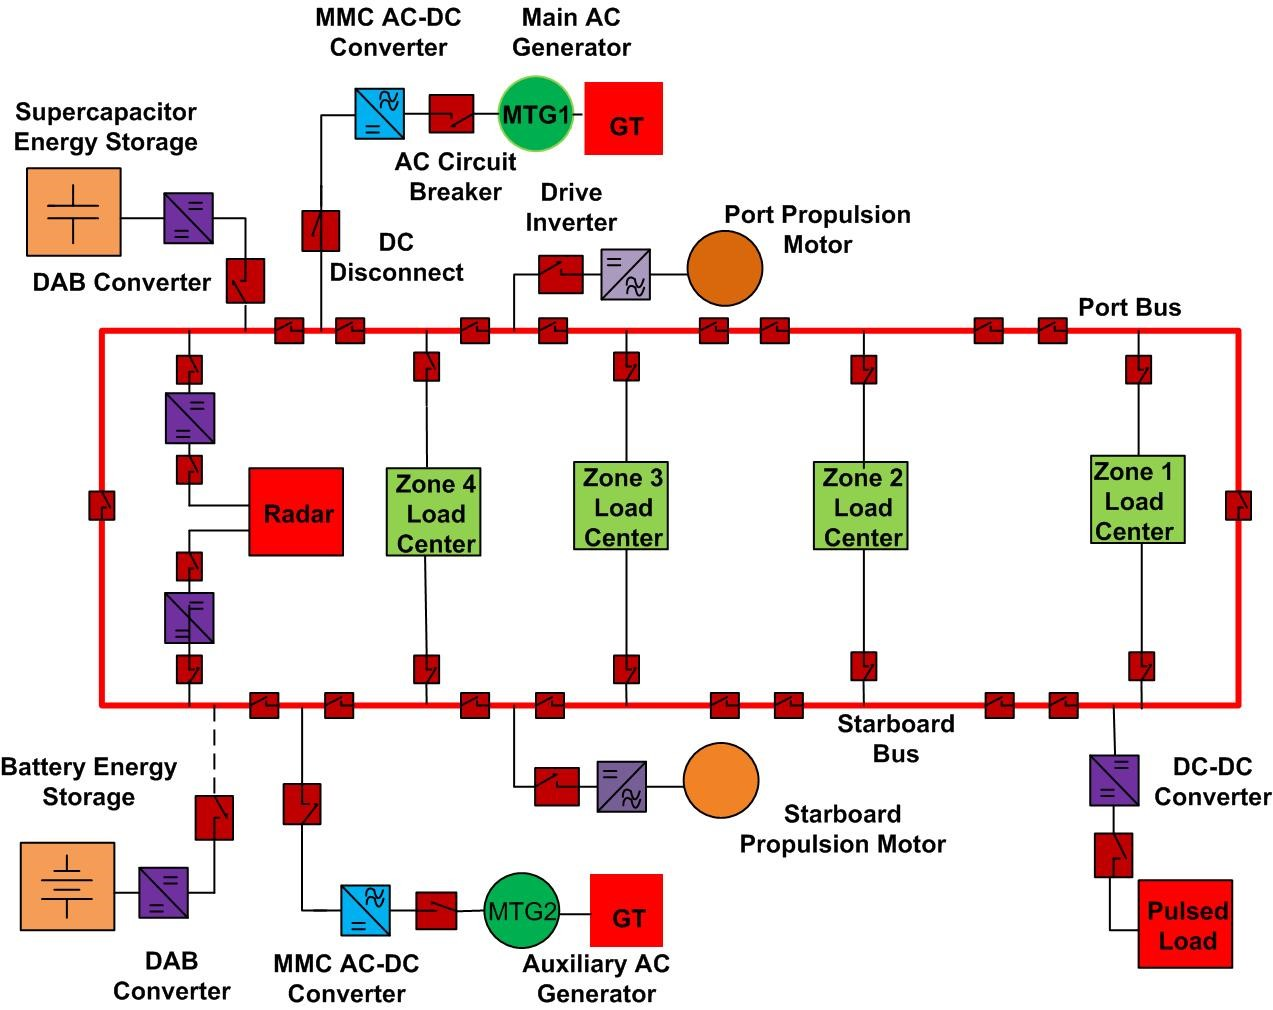
\includegraphics[width=\columnwidth]{f1}
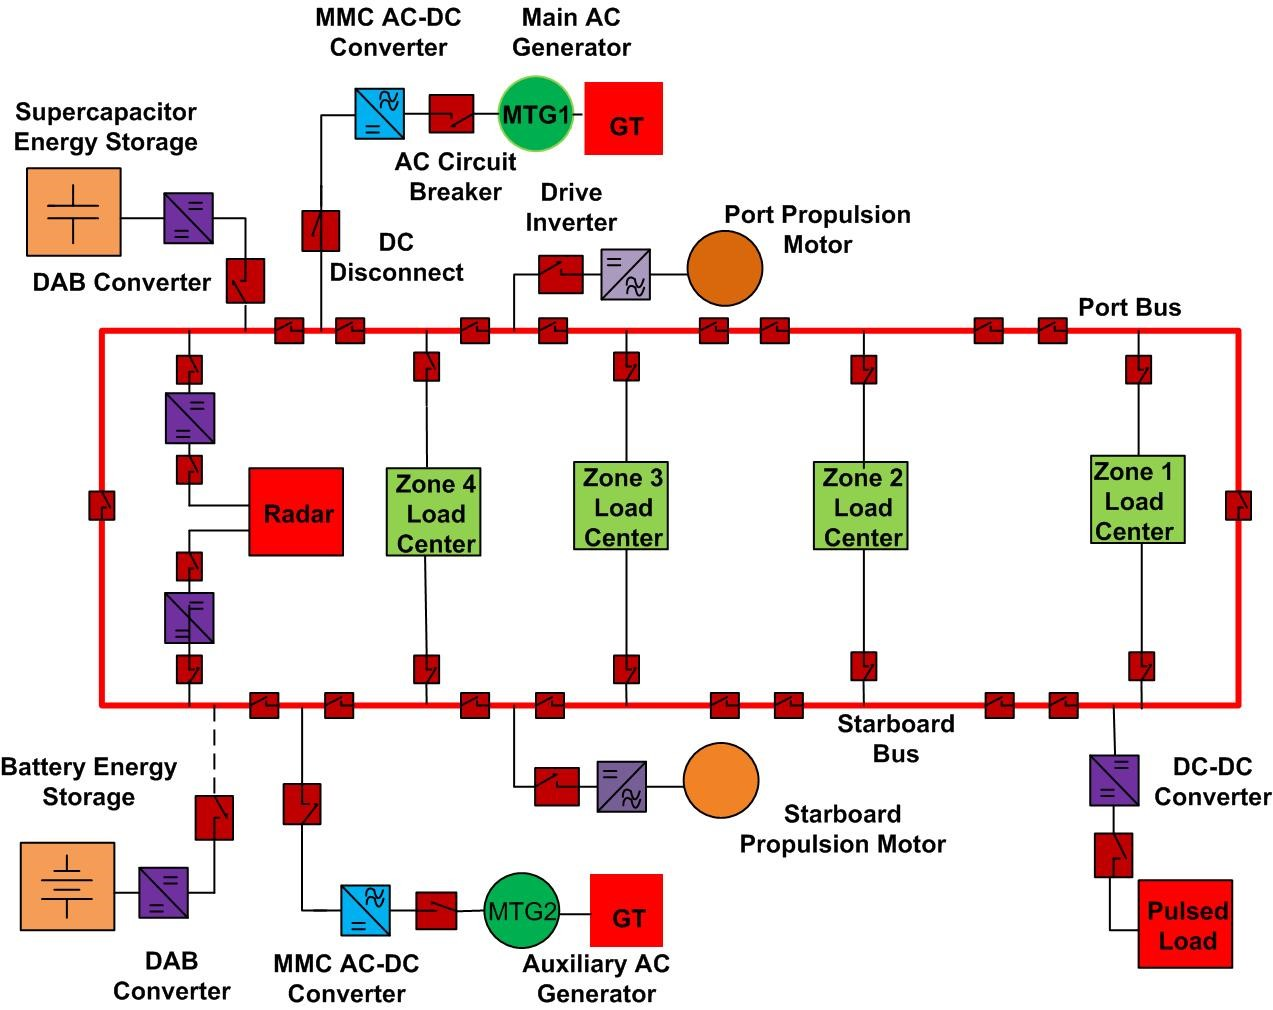
\includegraphics[width=3.46in, height=2.8in]{f1}
\caption{The 5kV MVDC system (40MW).}
\label{sec2_f1}
\end{figure}
%\vspace{-0.27in}